\documentclass[../../../../doc.tex]{subfiles}

\begin{document}
\subsection{Algorytm A*}

Algorytm A* jest algorytmem wyszukiwania ścieżki w grafie, który znajduje najkrótszą ścieżkę między punktem startowym a docelowym. Wykorzystuje funkcję heurystyczną do optymalizacji procesu przeszukiwania.

\subsubsection{Opis działania algorytmu}

Algorytm łączy zalety przeszukiwania wszerz (BFS) i zachłannego przeszukiwania najlepszego pierwszego (Best-First Search). Działa poprzez minimalizację funkcji kosztu:
\[
  f(n) = g(n) + h(n)
\]
gdzie:
\begin{itemize}
  \item $g(n)$ - rzeczywisty koszt dotarcia z węzła startowego do bieżącego
  \item $h(n)$ - heurystyczny koszt dotarcia z bieżącego węzła do celu
\end{itemize}

\subsubsection{Inicjalizacja}
\begin{enumerate}
  \item Inicjalizacja struktur danych:
        \begin{itemize}
          \item \texttt{state} - mapa stanów węzłów (przechowuje $g(n)$ i poprzednika)
          \item \texttt{sortedQueue} - kolejka priorytetowa węzłów (posortowana po $f(n)$)
        \end{itemize}
  \item Dodanie węzła startowego:
        \begin{itemize}
          \item $g(\text{start}) = 0$
          \item $f(\text{start}) = h(\text{start})$
          \item Oznaczenie startu jako \texttt{queued}
        \end{itemize}
\end{enumerate}

\subsubsection{Funkcja heurystyczna}
Wykorzystana heurystyka to \textbf{odległość Manhattan (Taxicab)}:
\[
  h(n) = |n_x - \text{end}_x| + |n_y - \text{end}_y|
\]
Zapewnia dopuszczalność (nie przeszacowuje kosztu).

\subsubsection{Główna pętla algorytmu}
\begin{algorithmic}
  \WHILE{kolejka nie jest pusta}
  \STATE Pobierz węzeł o minimalnym $f(n)$ z \texttt{sortedQueue}
  \STATE Oznacz bieżący węzeł jako \texttt{candidate}
  \IF{bieżący węzeł jest metą}
  \STATE Przerwij pętlę
  \ENDIF
  \FOR{każdego sąsiada}
  \IF{sąsiad nie jest kolizją i nie był odwiedzony}
  \STATE $g_{\text{new}} \gets g(\text{current}) + 1$
  \STATE $f_{\text{new}} \gets g_{\text{new}} + h(\text{sąsiad})$
  \STATE Zapisz stan: $g = g_{\text{new}}$, poprzednik = currentNodePos
  \STATE Wstaw do kolejki z priorytetem $f_{\text{new}}$
  \STATE Oznacz jako \texttt{queued}
  \ENDIF
  \ENDFOR
  \ENDWHILE
\end{algorithmic}

\subsubsection{Budowanie ścieżki}
\begin{enumerate}
  \item \textbf{Śledzenie wsteczne:}
        \begin{itemize}
          \item Rozpocznij od mety
          \item Podążaj do poprzedników aż do startu
          \item Oznaczaj węzły jako \texttt{selected}
        \end{itemize}
  \item \textbf{Końcowe przetwarzanie:}
        \begin{itemize}
          \item Odwróć ścieżkę (start $\rightarrow$ meta)
          \item Oznacz start jako \texttt{selected}
        \end{itemize}
\end{enumerate}


\subsubsection{Złożoność obliczeniowa}
\begin{itemize}
  \item \textbf{Czasowa}: $O(n^2)$ (dla implementacji z listą)
  \item \textbf{Pamięciowa}: $O(n)$ (przechowywanie stanów i kolejki)
\end{itemize}
Przykład działania algorytmu przedstawia \cref{fig:astar_solve_steps}.

\begin{multicols}{2}
  
        \begin{figure}[H]
          
          \centering
          
  \begin{tikzpicture}
  \fill[gray] (0, 0) rectangle (1, 1);
\fill[gray] (1, 0) rectangle (2, 1);
\fill[gray] (2, 0) rectangle (3, 1);
\fill[gray] (6, 0) rectangle (7, 1);
\node at (7.5, 0.5){\color{blue}\faIcon{home}};
\fill[gray] (8, 0) rectangle (9, 1);
\node at (1.5, 1.5){\color{blue}\faIcon{user}};
\fill[gray] (4, 1) rectangle (5, 2);
\fill[gray] (8, 1) rectangle (9, 2);
\fill[gray] (0, 2) rectangle (1, 3);
\fill[gray] (4, 2) rectangle (5, 3);
\fill[gray] (6, 2) rectangle (7, 3);
\fill[gray] (0, 3) rectangle (1, 4);
\fill[gray] (2, 3) rectangle (3, 4);
\fill[gray] (4, 3) rectangle (5, 4);
\fill[gray] (6, 3) rectangle (7, 4);
\fill[gray] (0, 4) rectangle (1, 5);
\fill[gray] (2, 4) rectangle (3, 5);
\fill[gray] (6, 4) rectangle (7, 5);
\fill[gray] (8, 4) rectangle (9, 5);
\fill[gray] (9, 4) rectangle (10, 5);
\draw[black] grid (10, 5);
  \end{tikzpicture}
  
          \caption{Dodaj do kolejki węzeł {"x":1,"y":1}}
          \label{fig:astar_solve_steps}
        \end{figure}
        
        \begin{figure}[H]
          \ContinuedFloat
          \centering
          
  \begin{tikzpicture}
  \fill[gray] (0, 0) rectangle (1, 1);
\fill[gray] (1, 0) rectangle (2, 1);
\fill[gray] (2, 0) rectangle (3, 1);
\fill[gray] (6, 0) rectangle (7, 1);
\node at (7.5, 0.5){\color{blue}\faIcon{home}};
\fill[gray] (8, 0) rectangle (9, 1);
\node at (1.5, 1.5){\color{blue}\faIcon{user}};
\fill[gray] (4, 1) rectangle (5, 2);
\fill[gray] (8, 1) rectangle (9, 2);
\fill[gray] (0, 2) rectangle (1, 3);
\fill[gray] (4, 2) rectangle (5, 3);
\fill[gray] (6, 2) rectangle (7, 3);
\fill[gray] (0, 3) rectangle (1, 4);
\fill[gray] (2, 3) rectangle (3, 4);
\fill[gray] (4, 3) rectangle (5, 4);
\fill[gray] (6, 3) rectangle (7, 4);
\fill[gray] (0, 4) rectangle (1, 5);
\fill[gray] (2, 4) rectangle (3, 5);
\fill[gray] (6, 4) rectangle (7, 5);
\fill[gray] (8, 4) rectangle (9, 5);
\fill[gray] (9, 4) rectangle (10, 5);
\draw[black] grid (10, 5);
  \end{tikzpicture}
  
          \caption{Rozpatrz {"x":1,"y":1}}
          
        \end{figure}
        
        \begin{figure}[H]
          \ContinuedFloat
          \centering
          
  \begin{tikzpicture}
  \fill[gray] (0, 0) rectangle (1, 1);
\fill[gray] (1, 0) rectangle (2, 1);
\fill[gray] (2, 0) rectangle (3, 1);
\fill[gray] (6, 0) rectangle (7, 1);
\node at (7.5, 0.5){\color{blue}\faIcon{home}};
\fill[gray] (8, 0) rectangle (9, 1);
\node at (0.5, 1.5){\color{purple}\faIcon{hourglass}};
\node at (1.5, 1.5){\color{blue}\faIcon{user}};
\fill[gray] (4, 1) rectangle (5, 2);
\fill[gray] (8, 1) rectangle (9, 2);
\fill[gray] (0, 2) rectangle (1, 3);
\fill[gray] (4, 2) rectangle (5, 3);
\fill[gray] (6, 2) rectangle (7, 3);
\fill[gray] (0, 3) rectangle (1, 4);
\fill[gray] (2, 3) rectangle (3, 4);
\fill[gray] (4, 3) rectangle (5, 4);
\fill[gray] (6, 3) rectangle (7, 4);
\fill[gray] (0, 4) rectangle (1, 5);
\fill[gray] (2, 4) rectangle (3, 5);
\fill[gray] (6, 4) rectangle (7, 5);
\fill[gray] (8, 4) rectangle (9, 5);
\fill[gray] (9, 4) rectangle (10, 5);
\draw[black] grid (10, 5);
  \end{tikzpicture}
  
          \caption{Dodaj do kolejki węzeł {"x":0,"y":1}}
          
        \end{figure}
        
        \begin{figure}[H]
          \ContinuedFloat
          \centering
          
  \begin{tikzpicture}
  \fill[gray] (0, 0) rectangle (1, 1);
\fill[gray] (1, 0) rectangle (2, 1);
\fill[gray] (2, 0) rectangle (3, 1);
\fill[gray] (6, 0) rectangle (7, 1);
\node at (7.5, 0.5){\color{blue}\faIcon{home}};
\fill[gray] (8, 0) rectangle (9, 1);
\node at (0.5, 1.5){\color{purple}\faIcon{hourglass}};
\node at (1.5, 1.5){\color{blue}\faIcon{user}};
\node at (2.5, 1.5){\color{purple}\faIcon{hourglass}};
\fill[gray] (4, 1) rectangle (5, 2);
\fill[gray] (8, 1) rectangle (9, 2);
\fill[gray] (0, 2) rectangle (1, 3);
\fill[gray] (4, 2) rectangle (5, 3);
\fill[gray] (6, 2) rectangle (7, 3);
\fill[gray] (0, 3) rectangle (1, 4);
\fill[gray] (2, 3) rectangle (3, 4);
\fill[gray] (4, 3) rectangle (5, 4);
\fill[gray] (6, 3) rectangle (7, 4);
\fill[gray] (0, 4) rectangle (1, 5);
\fill[gray] (2, 4) rectangle (3, 5);
\fill[gray] (6, 4) rectangle (7, 5);
\fill[gray] (8, 4) rectangle (9, 5);
\fill[gray] (9, 4) rectangle (10, 5);
\draw[black] grid (10, 5);
  \end{tikzpicture}
  
          \caption{Dodaj do kolejki węzeł {"x":2,"y":1}}
          
        \end{figure}
        
        \begin{figure}[H]
          \ContinuedFloat
          \centering
          
  \begin{tikzpicture}
  \fill[gray] (0, 0) rectangle (1, 1);
\fill[gray] (1, 0) rectangle (2, 1);
\fill[gray] (2, 0) rectangle (3, 1);
\fill[gray] (6, 0) rectangle (7, 1);
\node at (7.5, 0.5){\color{blue}\faIcon{home}};
\fill[gray] (8, 0) rectangle (9, 1);
\node at (0.5, 1.5){\color{purple}\faIcon{hourglass}};
\node at (1.5, 1.5){\color{blue}\faIcon{user}};
\node at (2.5, 1.5){\color{purple}\faIcon{hourglass}};
\fill[gray] (4, 1) rectangle (5, 2);
\fill[gray] (8, 1) rectangle (9, 2);
\fill[gray] (0, 2) rectangle (1, 3);
\node at (1.5, 2.5){\color{purple}\faIcon{hourglass}};
\fill[gray] (4, 2) rectangle (5, 3);
\fill[gray] (6, 2) rectangle (7, 3);
\fill[gray] (0, 3) rectangle (1, 4);
\fill[gray] (2, 3) rectangle (3, 4);
\fill[gray] (4, 3) rectangle (5, 4);
\fill[gray] (6, 3) rectangle (7, 4);
\fill[gray] (0, 4) rectangle (1, 5);
\fill[gray] (2, 4) rectangle (3, 5);
\fill[gray] (6, 4) rectangle (7, 5);
\fill[gray] (8, 4) rectangle (9, 5);
\fill[gray] (9, 4) rectangle (10, 5);
\draw[black] grid (10, 5);
  \end{tikzpicture}
  
          \caption{Dodaj do kolejki węzeł {"x":1,"y":2}}
          
        \end{figure}
        
        \begin{figure}[H]
          \ContinuedFloat
          \centering
          
  \begin{tikzpicture}
  \fill[gray] (0, 0) rectangle (1, 1);
\fill[gray] (1, 0) rectangle (2, 1);
\fill[gray] (2, 0) rectangle (3, 1);
\fill[gray] (6, 0) rectangle (7, 1);
\node at (7.5, 0.5){\color{blue}\faIcon{home}};
\fill[gray] (8, 0) rectangle (9, 1);
\node at (0.5, 1.5){\color{purple}\faIcon{hourglass}};
\node at (1.5, 1.5){\color{blue}\faIcon{user}};
\node at (2.5, 1.5){\color{orange}\faIcon{arrows-alt}};
\fill[gray] (4, 1) rectangle (5, 2);
\fill[gray] (8, 1) rectangle (9, 2);
\fill[gray] (0, 2) rectangle (1, 3);
\node at (1.5, 2.5){\color{purple}\faIcon{hourglass}};
\fill[gray] (4, 2) rectangle (5, 3);
\fill[gray] (6, 2) rectangle (7, 3);
\fill[gray] (0, 3) rectangle (1, 4);
\fill[gray] (2, 3) rectangle (3, 4);
\fill[gray] (4, 3) rectangle (5, 4);
\fill[gray] (6, 3) rectangle (7, 4);
\fill[gray] (0, 4) rectangle (1, 5);
\fill[gray] (2, 4) rectangle (3, 5);
\fill[gray] (6, 4) rectangle (7, 5);
\fill[gray] (8, 4) rectangle (9, 5);
\fill[gray] (9, 4) rectangle (10, 5);
\draw[black] grid (10, 5);
  \end{tikzpicture}
  
          \caption{Rozpatrz {"x":2,"y":1}}
          
        \end{figure}
        
        \begin{figure}[H]
          \ContinuedFloat
          \centering
          
  \begin{tikzpicture}
  \fill[gray] (0, 0) rectangle (1, 1);
\fill[gray] (1, 0) rectangle (2, 1);
\fill[gray] (2, 0) rectangle (3, 1);
\fill[gray] (6, 0) rectangle (7, 1);
\node at (7.5, 0.5){\color{blue}\faIcon{home}};
\fill[gray] (8, 0) rectangle (9, 1);
\node at (0.5, 1.5){\color{purple}\faIcon{hourglass}};
\node at (1.5, 1.5){\color{blue}\faIcon{user}};
\node at (2.5, 1.5){\color{orange}\faIcon{arrows-alt}};
\node at (3.5, 1.5){\color{purple}\faIcon{hourglass}};
\fill[gray] (4, 1) rectangle (5, 2);
\fill[gray] (8, 1) rectangle (9, 2);
\fill[gray] (0, 2) rectangle (1, 3);
\node at (1.5, 2.5){\color{purple}\faIcon{hourglass}};
\fill[gray] (4, 2) rectangle (5, 3);
\fill[gray] (6, 2) rectangle (7, 3);
\fill[gray] (0, 3) rectangle (1, 4);
\fill[gray] (2, 3) rectangle (3, 4);
\fill[gray] (4, 3) rectangle (5, 4);
\fill[gray] (6, 3) rectangle (7, 4);
\fill[gray] (0, 4) rectangle (1, 5);
\fill[gray] (2, 4) rectangle (3, 5);
\fill[gray] (6, 4) rectangle (7, 5);
\fill[gray] (8, 4) rectangle (9, 5);
\fill[gray] (9, 4) rectangle (10, 5);
\draw[black] grid (10, 5);
  \end{tikzpicture}
  
          \caption{Dodaj do kolejki węzeł {"x":3,"y":1}}
          
        \end{figure}
        
        \begin{figure}[H]
          \ContinuedFloat
          \centering
          
  \begin{tikzpicture}
  \fill[gray] (0, 0) rectangle (1, 1);
\fill[gray] (1, 0) rectangle (2, 1);
\fill[gray] (2, 0) rectangle (3, 1);
\fill[gray] (6, 0) rectangle (7, 1);
\node at (7.5, 0.5){\color{blue}\faIcon{home}};
\fill[gray] (8, 0) rectangle (9, 1);
\node at (0.5, 1.5){\color{purple}\faIcon{hourglass}};
\node at (1.5, 1.5){\color{blue}\faIcon{user}};
\node at (2.5, 1.5){\color{orange}\faIcon{arrows-alt}};
\node at (3.5, 1.5){\color{purple}\faIcon{hourglass}};
\fill[gray] (4, 1) rectangle (5, 2);
\fill[gray] (8, 1) rectangle (9, 2);
\fill[gray] (0, 2) rectangle (1, 3);
\node at (1.5, 2.5){\color{purple}\faIcon{hourglass}};
\node at (2.5, 2.5){\color{purple}\faIcon{hourglass}};
\fill[gray] (4, 2) rectangle (5, 3);
\fill[gray] (6, 2) rectangle (7, 3);
\fill[gray] (0, 3) rectangle (1, 4);
\fill[gray] (2, 3) rectangle (3, 4);
\fill[gray] (4, 3) rectangle (5, 4);
\fill[gray] (6, 3) rectangle (7, 4);
\fill[gray] (0, 4) rectangle (1, 5);
\fill[gray] (2, 4) rectangle (3, 5);
\fill[gray] (6, 4) rectangle (7, 5);
\fill[gray] (8, 4) rectangle (9, 5);
\fill[gray] (9, 4) rectangle (10, 5);
\draw[black] grid (10, 5);
  \end{tikzpicture}
  
          \caption{Dodaj do kolejki węzeł {"x":2,"y":2}}
          
        \end{figure}
        
        \begin{figure}[H]
          \ContinuedFloat
          \centering
          
  \begin{tikzpicture}
  \fill[gray] (0, 0) rectangle (1, 1);
\fill[gray] (1, 0) rectangle (2, 1);
\fill[gray] (2, 0) rectangle (3, 1);
\fill[gray] (6, 0) rectangle (7, 1);
\node at (7.5, 0.5){\color{blue}\faIcon{home}};
\fill[gray] (8, 0) rectangle (9, 1);
\node at (0.5, 1.5){\color{purple}\faIcon{hourglass}};
\node at (1.5, 1.5){\color{blue}\faIcon{user}};
\node at (2.5, 1.5){\color{orange}\faIcon{arrows-alt}};
\node at (3.5, 1.5){\color{orange}\faIcon{arrows-alt}};
\fill[gray] (4, 1) rectangle (5, 2);
\fill[gray] (8, 1) rectangle (9, 2);
\fill[gray] (0, 2) rectangle (1, 3);
\node at (1.5, 2.5){\color{purple}\faIcon{hourglass}};
\node at (2.5, 2.5){\color{purple}\faIcon{hourglass}};
\fill[gray] (4, 2) rectangle (5, 3);
\fill[gray] (6, 2) rectangle (7, 3);
\fill[gray] (0, 3) rectangle (1, 4);
\fill[gray] (2, 3) rectangle (3, 4);
\fill[gray] (4, 3) rectangle (5, 4);
\fill[gray] (6, 3) rectangle (7, 4);
\fill[gray] (0, 4) rectangle (1, 5);
\fill[gray] (2, 4) rectangle (3, 5);
\fill[gray] (6, 4) rectangle (7, 5);
\fill[gray] (8, 4) rectangle (9, 5);
\fill[gray] (9, 4) rectangle (10, 5);
\draw[black] grid (10, 5);
  \end{tikzpicture}
  
          \caption{Rozpatrz {"x":3,"y":1}}
          
        \end{figure}
        
        \begin{figure}[H]
          \ContinuedFloat
          \centering
          
  \begin{tikzpicture}
  \fill[gray] (0, 0) rectangle (1, 1);
\fill[gray] (1, 0) rectangle (2, 1);
\fill[gray] (2, 0) rectangle (3, 1);
\node at (3.5, 0.5){\color{purple}\faIcon{hourglass}};
\fill[gray] (6, 0) rectangle (7, 1);
\node at (7.5, 0.5){\color{blue}\faIcon{home}};
\fill[gray] (8, 0) rectangle (9, 1);
\node at (0.5, 1.5){\color{purple}\faIcon{hourglass}};
\node at (1.5, 1.5){\color{blue}\faIcon{user}};
\node at (2.5, 1.5){\color{orange}\faIcon{arrows-alt}};
\node at (3.5, 1.5){\color{orange}\faIcon{arrows-alt}};
\fill[gray] (4, 1) rectangle (5, 2);
\fill[gray] (8, 1) rectangle (9, 2);
\fill[gray] (0, 2) rectangle (1, 3);
\node at (1.5, 2.5){\color{purple}\faIcon{hourglass}};
\node at (2.5, 2.5){\color{purple}\faIcon{hourglass}};
\fill[gray] (4, 2) rectangle (5, 3);
\fill[gray] (6, 2) rectangle (7, 3);
\fill[gray] (0, 3) rectangle (1, 4);
\fill[gray] (2, 3) rectangle (3, 4);
\fill[gray] (4, 3) rectangle (5, 4);
\fill[gray] (6, 3) rectangle (7, 4);
\fill[gray] (0, 4) rectangle (1, 5);
\fill[gray] (2, 4) rectangle (3, 5);
\fill[gray] (6, 4) rectangle (7, 5);
\fill[gray] (8, 4) rectangle (9, 5);
\fill[gray] (9, 4) rectangle (10, 5);
\draw[black] grid (10, 5);
  \end{tikzpicture}
  
          \caption{Dodaj do kolejki węzeł {"x":3,"y":0}}
          
        \end{figure}
        
        \begin{figure}[H]
          \ContinuedFloat
          \centering
          
  \begin{tikzpicture}
  \fill[gray] (0, 0) rectangle (1, 1);
\fill[gray] (1, 0) rectangle (2, 1);
\fill[gray] (2, 0) rectangle (3, 1);
\node at (3.5, 0.5){\color{purple}\faIcon{hourglass}};
\fill[gray] (6, 0) rectangle (7, 1);
\node at (7.5, 0.5){\color{blue}\faIcon{home}};
\fill[gray] (8, 0) rectangle (9, 1);
\node at (0.5, 1.5){\color{purple}\faIcon{hourglass}};
\node at (1.5, 1.5){\color{blue}\faIcon{user}};
\node at (2.5, 1.5){\color{orange}\faIcon{arrows-alt}};
\node at (3.5, 1.5){\color{orange}\faIcon{arrows-alt}};
\fill[gray] (4, 1) rectangle (5, 2);
\fill[gray] (8, 1) rectangle (9, 2);
\fill[gray] (0, 2) rectangle (1, 3);
\node at (1.5, 2.5){\color{purple}\faIcon{hourglass}};
\node at (2.5, 2.5){\color{purple}\faIcon{hourglass}};
\node at (3.5, 2.5){\color{purple}\faIcon{hourglass}};
\fill[gray] (4, 2) rectangle (5, 3);
\fill[gray] (6, 2) rectangle (7, 3);
\fill[gray] (0, 3) rectangle (1, 4);
\fill[gray] (2, 3) rectangle (3, 4);
\fill[gray] (4, 3) rectangle (5, 4);
\fill[gray] (6, 3) rectangle (7, 4);
\fill[gray] (0, 4) rectangle (1, 5);
\fill[gray] (2, 4) rectangle (3, 5);
\fill[gray] (6, 4) rectangle (7, 5);
\fill[gray] (8, 4) rectangle (9, 5);
\fill[gray] (9, 4) rectangle (10, 5);
\draw[black] grid (10, 5);
  \end{tikzpicture}
  
          \caption{Dodaj do kolejki węzeł {"x":3,"y":2}}
          
        \end{figure}
        
        \begin{figure}[H]
          \ContinuedFloat
          \centering
          
  \begin{tikzpicture}
  \fill[gray] (0, 0) rectangle (1, 1);
\fill[gray] (1, 0) rectangle (2, 1);
\fill[gray] (2, 0) rectangle (3, 1);
\node at (3.5, 0.5){\color{orange}\faIcon{arrows-alt}};
\fill[gray] (6, 0) rectangle (7, 1);
\node at (7.5, 0.5){\color{blue}\faIcon{home}};
\fill[gray] (8, 0) rectangle (9, 1);
\node at (0.5, 1.5){\color{purple}\faIcon{hourglass}};
\node at (1.5, 1.5){\color{blue}\faIcon{user}};
\node at (2.5, 1.5){\color{orange}\faIcon{arrows-alt}};
\node at (3.5, 1.5){\color{orange}\faIcon{arrows-alt}};
\fill[gray] (4, 1) rectangle (5, 2);
\fill[gray] (8, 1) rectangle (9, 2);
\fill[gray] (0, 2) rectangle (1, 3);
\node at (1.5, 2.5){\color{purple}\faIcon{hourglass}};
\node at (2.5, 2.5){\color{purple}\faIcon{hourglass}};
\node at (3.5, 2.5){\color{purple}\faIcon{hourglass}};
\fill[gray] (4, 2) rectangle (5, 3);
\fill[gray] (6, 2) rectangle (7, 3);
\fill[gray] (0, 3) rectangle (1, 4);
\fill[gray] (2, 3) rectangle (3, 4);
\fill[gray] (4, 3) rectangle (5, 4);
\fill[gray] (6, 3) rectangle (7, 4);
\fill[gray] (0, 4) rectangle (1, 5);
\fill[gray] (2, 4) rectangle (3, 5);
\fill[gray] (6, 4) rectangle (7, 5);
\fill[gray] (8, 4) rectangle (9, 5);
\fill[gray] (9, 4) rectangle (10, 5);
\draw[black] grid (10, 5);
  \end{tikzpicture}
  
          \caption{Rozpatrz {"x":3,"y":0}}
          
        \end{figure}
        
        \begin{figure}[H]
          \ContinuedFloat
          \centering
          
  \begin{tikzpicture}
  \fill[gray] (0, 0) rectangle (1, 1);
\fill[gray] (1, 0) rectangle (2, 1);
\fill[gray] (2, 0) rectangle (3, 1);
\node at (3.5, 0.5){\color{orange}\faIcon{arrows-alt}};
\node at (4.5, 0.5){\color{purple}\faIcon{hourglass}};
\fill[gray] (6, 0) rectangle (7, 1);
\node at (7.5, 0.5){\color{blue}\faIcon{home}};
\fill[gray] (8, 0) rectangle (9, 1);
\node at (0.5, 1.5){\color{purple}\faIcon{hourglass}};
\node at (1.5, 1.5){\color{blue}\faIcon{user}};
\node at (2.5, 1.5){\color{orange}\faIcon{arrows-alt}};
\node at (3.5, 1.5){\color{orange}\faIcon{arrows-alt}};
\fill[gray] (4, 1) rectangle (5, 2);
\fill[gray] (8, 1) rectangle (9, 2);
\fill[gray] (0, 2) rectangle (1, 3);
\node at (1.5, 2.5){\color{purple}\faIcon{hourglass}};
\node at (2.5, 2.5){\color{purple}\faIcon{hourglass}};
\node at (3.5, 2.5){\color{purple}\faIcon{hourglass}};
\fill[gray] (4, 2) rectangle (5, 3);
\fill[gray] (6, 2) rectangle (7, 3);
\fill[gray] (0, 3) rectangle (1, 4);
\fill[gray] (2, 3) rectangle (3, 4);
\fill[gray] (4, 3) rectangle (5, 4);
\fill[gray] (6, 3) rectangle (7, 4);
\fill[gray] (0, 4) rectangle (1, 5);
\fill[gray] (2, 4) rectangle (3, 5);
\fill[gray] (6, 4) rectangle (7, 5);
\fill[gray] (8, 4) rectangle (9, 5);
\fill[gray] (9, 4) rectangle (10, 5);
\draw[black] grid (10, 5);
  \end{tikzpicture}
  
          \caption{Dodaj do kolejki węzeł {"x":4,"y":0}}
          
        \end{figure}
        
        \begin{figure}[H]
          \ContinuedFloat
          \centering
          
  \begin{tikzpicture}
  \fill[gray] (0, 0) rectangle (1, 1);
\fill[gray] (1, 0) rectangle (2, 1);
\fill[gray] (2, 0) rectangle (3, 1);
\node at (3.5, 0.5){\color{orange}\faIcon{arrows-alt}};
\node at (4.5, 0.5){\color{orange}\faIcon{arrows-alt}};
\fill[gray] (6, 0) rectangle (7, 1);
\node at (7.5, 0.5){\color{blue}\faIcon{home}};
\fill[gray] (8, 0) rectangle (9, 1);
\node at (0.5, 1.5){\color{purple}\faIcon{hourglass}};
\node at (1.5, 1.5){\color{blue}\faIcon{user}};
\node at (2.5, 1.5){\color{orange}\faIcon{arrows-alt}};
\node at (3.5, 1.5){\color{orange}\faIcon{arrows-alt}};
\fill[gray] (4, 1) rectangle (5, 2);
\fill[gray] (8, 1) rectangle (9, 2);
\fill[gray] (0, 2) rectangle (1, 3);
\node at (1.5, 2.5){\color{purple}\faIcon{hourglass}};
\node at (2.5, 2.5){\color{purple}\faIcon{hourglass}};
\node at (3.5, 2.5){\color{purple}\faIcon{hourglass}};
\fill[gray] (4, 2) rectangle (5, 3);
\fill[gray] (6, 2) rectangle (7, 3);
\fill[gray] (0, 3) rectangle (1, 4);
\fill[gray] (2, 3) rectangle (3, 4);
\fill[gray] (4, 3) rectangle (5, 4);
\fill[gray] (6, 3) rectangle (7, 4);
\fill[gray] (0, 4) rectangle (1, 5);
\fill[gray] (2, 4) rectangle (3, 5);
\fill[gray] (6, 4) rectangle (7, 5);
\fill[gray] (8, 4) rectangle (9, 5);
\fill[gray] (9, 4) rectangle (10, 5);
\draw[black] grid (10, 5);
  \end{tikzpicture}
  
          \caption{Rozpatrz {"x":4,"y":0}}
          
        \end{figure}
        
        \begin{figure}[H]
          \ContinuedFloat
          \centering
          
  \begin{tikzpicture}
  \fill[gray] (0, 0) rectangle (1, 1);
\fill[gray] (1, 0) rectangle (2, 1);
\fill[gray] (2, 0) rectangle (3, 1);
\node at (3.5, 0.5){\color{orange}\faIcon{arrows-alt}};
\node at (4.5, 0.5){\color{orange}\faIcon{arrows-alt}};
\node at (5.5, 0.5){\color{purple}\faIcon{hourglass}};
\fill[gray] (6, 0) rectangle (7, 1);
\node at (7.5, 0.5){\color{blue}\faIcon{home}};
\fill[gray] (8, 0) rectangle (9, 1);
\node at (0.5, 1.5){\color{purple}\faIcon{hourglass}};
\node at (1.5, 1.5){\color{blue}\faIcon{user}};
\node at (2.5, 1.5){\color{orange}\faIcon{arrows-alt}};
\node at (3.5, 1.5){\color{orange}\faIcon{arrows-alt}};
\fill[gray] (4, 1) rectangle (5, 2);
\fill[gray] (8, 1) rectangle (9, 2);
\fill[gray] (0, 2) rectangle (1, 3);
\node at (1.5, 2.5){\color{purple}\faIcon{hourglass}};
\node at (2.5, 2.5){\color{purple}\faIcon{hourglass}};
\node at (3.5, 2.5){\color{purple}\faIcon{hourglass}};
\fill[gray] (4, 2) rectangle (5, 3);
\fill[gray] (6, 2) rectangle (7, 3);
\fill[gray] (0, 3) rectangle (1, 4);
\fill[gray] (2, 3) rectangle (3, 4);
\fill[gray] (4, 3) rectangle (5, 4);
\fill[gray] (6, 3) rectangle (7, 4);
\fill[gray] (0, 4) rectangle (1, 5);
\fill[gray] (2, 4) rectangle (3, 5);
\fill[gray] (6, 4) rectangle (7, 5);
\fill[gray] (8, 4) rectangle (9, 5);
\fill[gray] (9, 4) rectangle (10, 5);
\draw[black] grid (10, 5);
  \end{tikzpicture}
  
          \caption{Dodaj do kolejki węzeł {"x":5,"y":0}}
          
        \end{figure}
        
        \begin{figure}[H]
          \ContinuedFloat
          \centering
          
  \begin{tikzpicture}
  \fill[gray] (0, 0) rectangle (1, 1);
\fill[gray] (1, 0) rectangle (2, 1);
\fill[gray] (2, 0) rectangle (3, 1);
\node at (3.5, 0.5){\color{orange}\faIcon{arrows-alt}};
\node at (4.5, 0.5){\color{orange}\faIcon{arrows-alt}};
\node at (5.5, 0.5){\color{orange}\faIcon{arrows-alt}};
\fill[gray] (6, 0) rectangle (7, 1);
\node at (7.5, 0.5){\color{blue}\faIcon{home}};
\fill[gray] (8, 0) rectangle (9, 1);
\node at (0.5, 1.5){\color{purple}\faIcon{hourglass}};
\node at (1.5, 1.5){\color{blue}\faIcon{user}};
\node at (2.5, 1.5){\color{orange}\faIcon{arrows-alt}};
\node at (3.5, 1.5){\color{orange}\faIcon{arrows-alt}};
\fill[gray] (4, 1) rectangle (5, 2);
\fill[gray] (8, 1) rectangle (9, 2);
\fill[gray] (0, 2) rectangle (1, 3);
\node at (1.5, 2.5){\color{purple}\faIcon{hourglass}};
\node at (2.5, 2.5){\color{purple}\faIcon{hourglass}};
\node at (3.5, 2.5){\color{purple}\faIcon{hourglass}};
\fill[gray] (4, 2) rectangle (5, 3);
\fill[gray] (6, 2) rectangle (7, 3);
\fill[gray] (0, 3) rectangle (1, 4);
\fill[gray] (2, 3) rectangle (3, 4);
\fill[gray] (4, 3) rectangle (5, 4);
\fill[gray] (6, 3) rectangle (7, 4);
\fill[gray] (0, 4) rectangle (1, 5);
\fill[gray] (2, 4) rectangle (3, 5);
\fill[gray] (6, 4) rectangle (7, 5);
\fill[gray] (8, 4) rectangle (9, 5);
\fill[gray] (9, 4) rectangle (10, 5);
\draw[black] grid (10, 5);
  \end{tikzpicture}
  
          \caption{Rozpatrz {"x":5,"y":0}}
          
        \end{figure}
        
        \begin{figure}[H]
          \ContinuedFloat
          \centering
          
  \begin{tikzpicture}
  \fill[gray] (0, 0) rectangle (1, 1);
\fill[gray] (1, 0) rectangle (2, 1);
\fill[gray] (2, 0) rectangle (3, 1);
\node at (3.5, 0.5){\color{orange}\faIcon{arrows-alt}};
\node at (4.5, 0.5){\color{orange}\faIcon{arrows-alt}};
\node at (5.5, 0.5){\color{orange}\faIcon{arrows-alt}};
\fill[gray] (6, 0) rectangle (7, 1);
\node at (7.5, 0.5){\color{blue}\faIcon{home}};
\fill[gray] (8, 0) rectangle (9, 1);
\node at (0.5, 1.5){\color{purple}\faIcon{hourglass}};
\node at (1.5, 1.5){\color{blue}\faIcon{user}};
\node at (2.5, 1.5){\color{orange}\faIcon{arrows-alt}};
\node at (3.5, 1.5){\color{orange}\faIcon{arrows-alt}};
\fill[gray] (4, 1) rectangle (5, 2);
\node at (5.5, 1.5){\color{purple}\faIcon{hourglass}};
\fill[gray] (8, 1) rectangle (9, 2);
\fill[gray] (0, 2) rectangle (1, 3);
\node at (1.5, 2.5){\color{purple}\faIcon{hourglass}};
\node at (2.5, 2.5){\color{purple}\faIcon{hourglass}};
\node at (3.5, 2.5){\color{purple}\faIcon{hourglass}};
\fill[gray] (4, 2) rectangle (5, 3);
\fill[gray] (6, 2) rectangle (7, 3);
\fill[gray] (0, 3) rectangle (1, 4);
\fill[gray] (2, 3) rectangle (3, 4);
\fill[gray] (4, 3) rectangle (5, 4);
\fill[gray] (6, 3) rectangle (7, 4);
\fill[gray] (0, 4) rectangle (1, 5);
\fill[gray] (2, 4) rectangle (3, 5);
\fill[gray] (6, 4) rectangle (7, 5);
\fill[gray] (8, 4) rectangle (9, 5);
\fill[gray] (9, 4) rectangle (10, 5);
\draw[black] grid (10, 5);
  \end{tikzpicture}
  
          \caption{Dodaj do kolejki węzeł {"x":5,"y":1}}
          
        \end{figure}
        
        \begin{figure}[H]
          \ContinuedFloat
          \centering
          
  \begin{tikzpicture}
  \fill[gray] (0, 0) rectangle (1, 1);
\fill[gray] (1, 0) rectangle (2, 1);
\fill[gray] (2, 0) rectangle (3, 1);
\node at (3.5, 0.5){\color{orange}\faIcon{arrows-alt}};
\node at (4.5, 0.5){\color{orange}\faIcon{arrows-alt}};
\node at (5.5, 0.5){\color{orange}\faIcon{arrows-alt}};
\fill[gray] (6, 0) rectangle (7, 1);
\node at (7.5, 0.5){\color{blue}\faIcon{home}};
\fill[gray] (8, 0) rectangle (9, 1);
\node at (0.5, 1.5){\color{purple}\faIcon{hourglass}};
\node at (1.5, 1.5){\color{blue}\faIcon{user}};
\node at (2.5, 1.5){\color{orange}\faIcon{arrows-alt}};
\node at (3.5, 1.5){\color{orange}\faIcon{arrows-alt}};
\fill[gray] (4, 1) rectangle (5, 2);
\node at (5.5, 1.5){\color{orange}\faIcon{arrows-alt}};
\fill[gray] (8, 1) rectangle (9, 2);
\fill[gray] (0, 2) rectangle (1, 3);
\node at (1.5, 2.5){\color{purple}\faIcon{hourglass}};
\node at (2.5, 2.5){\color{purple}\faIcon{hourglass}};
\node at (3.5, 2.5){\color{purple}\faIcon{hourglass}};
\fill[gray] (4, 2) rectangle (5, 3);
\fill[gray] (6, 2) rectangle (7, 3);
\fill[gray] (0, 3) rectangle (1, 4);
\fill[gray] (2, 3) rectangle (3, 4);
\fill[gray] (4, 3) rectangle (5, 4);
\fill[gray] (6, 3) rectangle (7, 4);
\fill[gray] (0, 4) rectangle (1, 5);
\fill[gray] (2, 4) rectangle (3, 5);
\fill[gray] (6, 4) rectangle (7, 5);
\fill[gray] (8, 4) rectangle (9, 5);
\fill[gray] (9, 4) rectangle (10, 5);
\draw[black] grid (10, 5);
  \end{tikzpicture}
  
          \caption{Rozpatrz {"x":5,"y":1}}
          
        \end{figure}
        
        \begin{figure}[H]
          \ContinuedFloat
          \centering
          
  \begin{tikzpicture}
  \fill[gray] (0, 0) rectangle (1, 1);
\fill[gray] (1, 0) rectangle (2, 1);
\fill[gray] (2, 0) rectangle (3, 1);
\node at (3.5, 0.5){\color{orange}\faIcon{arrows-alt}};
\node at (4.5, 0.5){\color{orange}\faIcon{arrows-alt}};
\node at (5.5, 0.5){\color{orange}\faIcon{arrows-alt}};
\fill[gray] (6, 0) rectangle (7, 1);
\node at (7.5, 0.5){\color{blue}\faIcon{home}};
\fill[gray] (8, 0) rectangle (9, 1);
\node at (0.5, 1.5){\color{purple}\faIcon{hourglass}};
\node at (1.5, 1.5){\color{blue}\faIcon{user}};
\node at (2.5, 1.5){\color{orange}\faIcon{arrows-alt}};
\node at (3.5, 1.5){\color{orange}\faIcon{arrows-alt}};
\fill[gray] (4, 1) rectangle (5, 2);
\node at (5.5, 1.5){\color{orange}\faIcon{arrows-alt}};
\node at (6.5, 1.5){\color{purple}\faIcon{hourglass}};
\fill[gray] (8, 1) rectangle (9, 2);
\fill[gray] (0, 2) rectangle (1, 3);
\node at (1.5, 2.5){\color{purple}\faIcon{hourglass}};
\node at (2.5, 2.5){\color{purple}\faIcon{hourglass}};
\node at (3.5, 2.5){\color{purple}\faIcon{hourglass}};
\fill[gray] (4, 2) rectangle (5, 3);
\fill[gray] (6, 2) rectangle (7, 3);
\fill[gray] (0, 3) rectangle (1, 4);
\fill[gray] (2, 3) rectangle (3, 4);
\fill[gray] (4, 3) rectangle (5, 4);
\fill[gray] (6, 3) rectangle (7, 4);
\fill[gray] (0, 4) rectangle (1, 5);
\fill[gray] (2, 4) rectangle (3, 5);
\fill[gray] (6, 4) rectangle (7, 5);
\fill[gray] (8, 4) rectangle (9, 5);
\fill[gray] (9, 4) rectangle (10, 5);
\draw[black] grid (10, 5);
  \end{tikzpicture}
  
          \caption{Dodaj do kolejki węzeł {"x":6,"y":1}}
          
        \end{figure}
        
        \begin{figure}[H]
          \ContinuedFloat
          \centering
          
  \begin{tikzpicture}
  \fill[gray] (0, 0) rectangle (1, 1);
\fill[gray] (1, 0) rectangle (2, 1);
\fill[gray] (2, 0) rectangle (3, 1);
\node at (3.5, 0.5){\color{orange}\faIcon{arrows-alt}};
\node at (4.5, 0.5){\color{orange}\faIcon{arrows-alt}};
\node at (5.5, 0.5){\color{orange}\faIcon{arrows-alt}};
\fill[gray] (6, 0) rectangle (7, 1);
\node at (7.5, 0.5){\color{blue}\faIcon{home}};
\fill[gray] (8, 0) rectangle (9, 1);
\node at (0.5, 1.5){\color{purple}\faIcon{hourglass}};
\node at (1.5, 1.5){\color{blue}\faIcon{user}};
\node at (2.5, 1.5){\color{orange}\faIcon{arrows-alt}};
\node at (3.5, 1.5){\color{orange}\faIcon{arrows-alt}};
\fill[gray] (4, 1) rectangle (5, 2);
\node at (5.5, 1.5){\color{orange}\faIcon{arrows-alt}};
\node at (6.5, 1.5){\color{purple}\faIcon{hourglass}};
\fill[gray] (8, 1) rectangle (9, 2);
\fill[gray] (0, 2) rectangle (1, 3);
\node at (1.5, 2.5){\color{purple}\faIcon{hourglass}};
\node at (2.5, 2.5){\color{purple}\faIcon{hourglass}};
\node at (3.5, 2.5){\color{purple}\faIcon{hourglass}};
\fill[gray] (4, 2) rectangle (5, 3);
\node at (5.5, 2.5){\color{purple}\faIcon{hourglass}};
\fill[gray] (6, 2) rectangle (7, 3);
\fill[gray] (0, 3) rectangle (1, 4);
\fill[gray] (2, 3) rectangle (3, 4);
\fill[gray] (4, 3) rectangle (5, 4);
\fill[gray] (6, 3) rectangle (7, 4);
\fill[gray] (0, 4) rectangle (1, 5);
\fill[gray] (2, 4) rectangle (3, 5);
\fill[gray] (6, 4) rectangle (7, 5);
\fill[gray] (8, 4) rectangle (9, 5);
\fill[gray] (9, 4) rectangle (10, 5);
\draw[black] grid (10, 5);
  \end{tikzpicture}
  
          \caption{Dodaj do kolejki węzeł {"x":5,"y":2}}
          
        \end{figure}
        
        \begin{figure}[H]
          \ContinuedFloat
          \centering
          
  \begin{tikzpicture}
  \fill[gray] (0, 0) rectangle (1, 1);
\fill[gray] (1, 0) rectangle (2, 1);
\fill[gray] (2, 0) rectangle (3, 1);
\node at (3.5, 0.5){\color{orange}\faIcon{arrows-alt}};
\node at (4.5, 0.5){\color{orange}\faIcon{arrows-alt}};
\node at (5.5, 0.5){\color{orange}\faIcon{arrows-alt}};
\fill[gray] (6, 0) rectangle (7, 1);
\node at (7.5, 0.5){\color{blue}\faIcon{home}};
\fill[gray] (8, 0) rectangle (9, 1);
\node at (0.5, 1.5){\color{purple}\faIcon{hourglass}};
\node at (1.5, 1.5){\color{blue}\faIcon{user}};
\node at (2.5, 1.5){\color{orange}\faIcon{arrows-alt}};
\node at (3.5, 1.5){\color{orange}\faIcon{arrows-alt}};
\fill[gray] (4, 1) rectangle (5, 2);
\node at (5.5, 1.5){\color{orange}\faIcon{arrows-alt}};
\node at (6.5, 1.5){\color{orange}\faIcon{arrows-alt}};
\fill[gray] (8, 1) rectangle (9, 2);
\fill[gray] (0, 2) rectangle (1, 3);
\node at (1.5, 2.5){\color{purple}\faIcon{hourglass}};
\node at (2.5, 2.5){\color{purple}\faIcon{hourglass}};
\node at (3.5, 2.5){\color{purple}\faIcon{hourglass}};
\fill[gray] (4, 2) rectangle (5, 3);
\node at (5.5, 2.5){\color{purple}\faIcon{hourglass}};
\fill[gray] (6, 2) rectangle (7, 3);
\fill[gray] (0, 3) rectangle (1, 4);
\fill[gray] (2, 3) rectangle (3, 4);
\fill[gray] (4, 3) rectangle (5, 4);
\fill[gray] (6, 3) rectangle (7, 4);
\fill[gray] (0, 4) rectangle (1, 5);
\fill[gray] (2, 4) rectangle (3, 5);
\fill[gray] (6, 4) rectangle (7, 5);
\fill[gray] (8, 4) rectangle (9, 5);
\fill[gray] (9, 4) rectangle (10, 5);
\draw[black] grid (10, 5);
  \end{tikzpicture}
  
          \caption{Rozpatrz {"x":6,"y":1}}
          
        \end{figure}
        
        \begin{figure}[H]
          \ContinuedFloat
          \centering
          
  \begin{tikzpicture}
  \fill[gray] (0, 0) rectangle (1, 1);
\fill[gray] (1, 0) rectangle (2, 1);
\fill[gray] (2, 0) rectangle (3, 1);
\node at (3.5, 0.5){\color{orange}\faIcon{arrows-alt}};
\node at (4.5, 0.5){\color{orange}\faIcon{arrows-alt}};
\node at (5.5, 0.5){\color{orange}\faIcon{arrows-alt}};
\fill[gray] (6, 0) rectangle (7, 1);
\node at (7.5, 0.5){\color{blue}\faIcon{home}};
\fill[gray] (8, 0) rectangle (9, 1);
\node at (0.5, 1.5){\color{purple}\faIcon{hourglass}};
\node at (1.5, 1.5){\color{blue}\faIcon{user}};
\node at (2.5, 1.5){\color{orange}\faIcon{arrows-alt}};
\node at (3.5, 1.5){\color{orange}\faIcon{arrows-alt}};
\fill[gray] (4, 1) rectangle (5, 2);
\node at (5.5, 1.5){\color{orange}\faIcon{arrows-alt}};
\node at (6.5, 1.5){\color{orange}\faIcon{arrows-alt}};
\node at (7.5, 1.5){\color{purple}\faIcon{hourglass}};
\fill[gray] (8, 1) rectangle (9, 2);
\fill[gray] (0, 2) rectangle (1, 3);
\node at (1.5, 2.5){\color{purple}\faIcon{hourglass}};
\node at (2.5, 2.5){\color{purple}\faIcon{hourglass}};
\node at (3.5, 2.5){\color{purple}\faIcon{hourglass}};
\fill[gray] (4, 2) rectangle (5, 3);
\node at (5.5, 2.5){\color{purple}\faIcon{hourglass}};
\fill[gray] (6, 2) rectangle (7, 3);
\fill[gray] (0, 3) rectangle (1, 4);
\fill[gray] (2, 3) rectangle (3, 4);
\fill[gray] (4, 3) rectangle (5, 4);
\fill[gray] (6, 3) rectangle (7, 4);
\fill[gray] (0, 4) rectangle (1, 5);
\fill[gray] (2, 4) rectangle (3, 5);
\fill[gray] (6, 4) rectangle (7, 5);
\fill[gray] (8, 4) rectangle (9, 5);
\fill[gray] (9, 4) rectangle (10, 5);
\draw[black] grid (10, 5);
  \end{tikzpicture}
  
          \caption{Dodaj do kolejki węzeł {"x":7,"y":1}}
          
        \end{figure}
        
        \begin{figure}[H]
          \ContinuedFloat
          \centering
          
  \begin{tikzpicture}
  \fill[gray] (0, 0) rectangle (1, 1);
\fill[gray] (1, 0) rectangle (2, 1);
\fill[gray] (2, 0) rectangle (3, 1);
\node at (3.5, 0.5){\color{orange}\faIcon{arrows-alt}};
\node at (4.5, 0.5){\color{orange}\faIcon{arrows-alt}};
\node at (5.5, 0.5){\color{orange}\faIcon{arrows-alt}};
\fill[gray] (6, 0) rectangle (7, 1);
\node at (7.5, 0.5){\color{blue}\faIcon{home}};
\fill[gray] (8, 0) rectangle (9, 1);
\node at (0.5, 1.5){\color{purple}\faIcon{hourglass}};
\node at (1.5, 1.5){\color{blue}\faIcon{user}};
\node at (2.5, 1.5){\color{orange}\faIcon{arrows-alt}};
\node at (3.5, 1.5){\color{orange}\faIcon{arrows-alt}};
\fill[gray] (4, 1) rectangle (5, 2);
\node at (5.5, 1.5){\color{orange}\faIcon{arrows-alt}};
\node at (6.5, 1.5){\color{orange}\faIcon{arrows-alt}};
\node at (7.5, 1.5){\color{orange}\faIcon{arrows-alt}};
\fill[gray] (8, 1) rectangle (9, 2);
\fill[gray] (0, 2) rectangle (1, 3);
\node at (1.5, 2.5){\color{purple}\faIcon{hourglass}};
\node at (2.5, 2.5){\color{purple}\faIcon{hourglass}};
\node at (3.5, 2.5){\color{purple}\faIcon{hourglass}};
\fill[gray] (4, 2) rectangle (5, 3);
\node at (5.5, 2.5){\color{purple}\faIcon{hourglass}};
\fill[gray] (6, 2) rectangle (7, 3);
\fill[gray] (0, 3) rectangle (1, 4);
\fill[gray] (2, 3) rectangle (3, 4);
\fill[gray] (4, 3) rectangle (5, 4);
\fill[gray] (6, 3) rectangle (7, 4);
\fill[gray] (0, 4) rectangle (1, 5);
\fill[gray] (2, 4) rectangle (3, 5);
\fill[gray] (6, 4) rectangle (7, 5);
\fill[gray] (8, 4) rectangle (9, 5);
\fill[gray] (9, 4) rectangle (10, 5);
\draw[black] grid (10, 5);
  \end{tikzpicture}
  
          \caption{Rozpatrz {"x":7,"y":1}}
          
        \end{figure}
        
        \begin{figure}[H]
          \ContinuedFloat
          \centering
          
  \begin{tikzpicture}
  \fill[gray] (0, 0) rectangle (1, 1);
\fill[gray] (1, 0) rectangle (2, 1);
\fill[gray] (2, 0) rectangle (3, 1);
\node at (3.5, 0.5){\color{orange}\faIcon{arrows-alt}};
\node at (4.5, 0.5){\color{orange}\faIcon{arrows-alt}};
\node at (5.5, 0.5){\color{orange}\faIcon{arrows-alt}};
\fill[gray] (6, 0) rectangle (7, 1);
\node at (7.5, 0.5){\color{blue}\faIcon{home}};
\fill[gray] (8, 0) rectangle (9, 1);
\node at (0.5, 1.5){\color{purple}\faIcon{hourglass}};
\node at (1.5, 1.5){\color{blue}\faIcon{user}};
\node at (2.5, 1.5){\color{orange}\faIcon{arrows-alt}};
\node at (3.5, 1.5){\color{orange}\faIcon{arrows-alt}};
\fill[gray] (4, 1) rectangle (5, 2);
\node at (5.5, 1.5){\color{orange}\faIcon{arrows-alt}};
\node at (6.5, 1.5){\color{orange}\faIcon{arrows-alt}};
\node at (7.5, 1.5){\color{orange}\faIcon{arrows-alt}};
\fill[gray] (8, 1) rectangle (9, 2);
\fill[gray] (0, 2) rectangle (1, 3);
\node at (1.5, 2.5){\color{purple}\faIcon{hourglass}};
\node at (2.5, 2.5){\color{purple}\faIcon{hourglass}};
\node at (3.5, 2.5){\color{purple}\faIcon{hourglass}};
\fill[gray] (4, 2) rectangle (5, 3);
\node at (5.5, 2.5){\color{purple}\faIcon{hourglass}};
\fill[gray] (6, 2) rectangle (7, 3);
\node at (7.5, 2.5){\color{purple}\faIcon{hourglass}};
\fill[gray] (0, 3) rectangle (1, 4);
\fill[gray] (2, 3) rectangle (3, 4);
\fill[gray] (4, 3) rectangle (5, 4);
\fill[gray] (6, 3) rectangle (7, 4);
\fill[gray] (0, 4) rectangle (1, 5);
\fill[gray] (2, 4) rectangle (3, 5);
\fill[gray] (6, 4) rectangle (7, 5);
\fill[gray] (8, 4) rectangle (9, 5);
\fill[gray] (9, 4) rectangle (10, 5);
\draw[black] grid (10, 5);
  \end{tikzpicture}
  
          \caption{Dodaj do kolejki węzeł {"x":7,"y":2}}
          
        \end{figure}
        
        \begin{figure}[H]
          \ContinuedFloat
          \centering
          
  \begin{tikzpicture}
  \fill[gray] (0, 0) rectangle (1, 1);
\fill[gray] (1, 0) rectangle (2, 1);
\fill[gray] (2, 0) rectangle (3, 1);
\node at (3.5, 0.5){\color{orange}\faIcon{arrows-alt}};
\node at (4.5, 0.5){\color{orange}\faIcon{arrows-alt}};
\node at (5.5, 0.5){\color{orange}\faIcon{arrows-alt}};
\fill[gray] (6, 0) rectangle (7, 1);
\node at (7.5, 0.5){\color{blue}\faIcon{home}};
\fill[gray] (8, 0) rectangle (9, 1);
\node at (0.5, 1.5){\color{purple}\faIcon{hourglass}};
\node at (1.5, 1.5){\color{blue}\faIcon{user}};
\node at (2.5, 1.5){\color{orange}\faIcon{arrows-alt}};
\node at (3.5, 1.5){\color{orange}\faIcon{arrows-alt}};
\fill[gray] (4, 1) rectangle (5, 2);
\node at (5.5, 1.5){\color{orange}\faIcon{arrows-alt}};
\node at (6.5, 1.5){\color{orange}\faIcon{arrows-alt}};
\node at (7.5, 1.5){\color{orange}\faIcon{arrows-alt}};
\fill[gray] (8, 1) rectangle (9, 2);
\fill[gray] (0, 2) rectangle (1, 3);
\node at (1.5, 2.5){\color{purple}\faIcon{hourglass}};
\node at (2.5, 2.5){\color{purple}\faIcon{hourglass}};
\node at (3.5, 2.5){\color{purple}\faIcon{hourglass}};
\fill[gray] (4, 2) rectangle (5, 3);
\node at (5.5, 2.5){\color{purple}\faIcon{hourglass}};
\fill[gray] (6, 2) rectangle (7, 3);
\node at (7.5, 2.5){\color{purple}\faIcon{hourglass}};
\fill[gray] (0, 3) rectangle (1, 4);
\fill[gray] (2, 3) rectangle (3, 4);
\fill[gray] (4, 3) rectangle (5, 4);
\fill[gray] (6, 3) rectangle (7, 4);
\fill[gray] (0, 4) rectangle (1, 5);
\fill[gray] (2, 4) rectangle (3, 5);
\fill[gray] (6, 4) rectangle (7, 5);
\fill[gray] (8, 4) rectangle (9, 5);
\fill[gray] (9, 4) rectangle (10, 5);
\draw[black] grid (10, 5);
  \end{tikzpicture}
  
          \caption{Dodaj do kolejki węzeł {"x":7,"y":0}}
          
        \end{figure}
        
        \begin{figure}[H]
          \ContinuedFloat
          \centering
          
  \begin{tikzpicture}
  \fill[gray] (0, 0) rectangle (1, 1);
\fill[gray] (1, 0) rectangle (2, 1);
\fill[gray] (2, 0) rectangle (3, 1);
\node at (3.5, 0.5){\color{orange}\faIcon{arrows-alt}};
\node at (4.5, 0.5){\color{orange}\faIcon{arrows-alt}};
\node at (5.5, 0.5){\color{orange}\faIcon{arrows-alt}};
\fill[gray] (6, 0) rectangle (7, 1);
\node at (7.5, 0.5){\color{blue}\faIcon{home}};
\fill[gray] (8, 0) rectangle (9, 1);
\node at (0.5, 1.5){\color{purple}\faIcon{hourglass}};
\node at (1.5, 1.5){\color{blue}\faIcon{user}};
\node at (2.5, 1.5){\color{orange}\faIcon{arrows-alt}};
\node at (3.5, 1.5){\color{orange}\faIcon{arrows-alt}};
\fill[gray] (4, 1) rectangle (5, 2);
\node at (5.5, 1.5){\color{orange}\faIcon{arrows-alt}};
\node at (6.5, 1.5){\color{orange}\faIcon{arrows-alt}};
\node at (7.5, 1.5){\color{orange}\faIcon{arrows-alt}};
\fill[gray] (8, 1) rectangle (9, 2);
\fill[gray] (0, 2) rectangle (1, 3);
\node at (1.5, 2.5){\color{purple}\faIcon{hourglass}};
\node at (2.5, 2.5){\color{purple}\faIcon{hourglass}};
\node at (3.5, 2.5){\color{purple}\faIcon{hourglass}};
\fill[gray] (4, 2) rectangle (5, 3);
\node at (5.5, 2.5){\color{purple}\faIcon{hourglass}};
\fill[gray] (6, 2) rectangle (7, 3);
\node at (7.5, 2.5){\color{purple}\faIcon{hourglass}};
\fill[gray] (0, 3) rectangle (1, 4);
\fill[gray] (2, 3) rectangle (3, 4);
\fill[gray] (4, 3) rectangle (5, 4);
\fill[gray] (6, 3) rectangle (7, 4);
\fill[gray] (0, 4) rectangle (1, 5);
\fill[gray] (2, 4) rectangle (3, 5);
\fill[gray] (6, 4) rectangle (7, 5);
\fill[gray] (8, 4) rectangle (9, 5);
\fill[gray] (9, 4) rectangle (10, 5);
\draw[black] grid (10, 5);
  \end{tikzpicture}
  
          \caption{Rozpatrz {"x":7,"y":0}}
          
        \end{figure}
        
        \begin{figure}[H]
          \ContinuedFloat
          \centering
          
  \begin{tikzpicture}
  \fill[gray] (0, 0) rectangle (1, 1);
\fill[gray] (1, 0) rectangle (2, 1);
\fill[gray] (2, 0) rectangle (3, 1);
\node at (3.5, 0.5){\color{orange}\faIcon{arrows-alt}};
\node at (4.5, 0.5){\color{orange}\faIcon{arrows-alt}};
\node at (5.5, 0.5){\color{orange}\faIcon{arrows-alt}};
\fill[gray] (6, 0) rectangle (7, 1);
\node at (7.5, 0.5){\color{blue}\faIcon{home}};
\fill[gray] (8, 0) rectangle (9, 1);
\node at (0.5, 1.5){\color{purple}\faIcon{hourglass}};
\node at (1.5, 1.5){\color{blue}\faIcon{user}};
\node at (2.5, 1.5){\color{orange}\faIcon{arrows-alt}};
\node at (3.5, 1.5){\color{orange}\faIcon{arrows-alt}};
\fill[gray] (4, 1) rectangle (5, 2);
\node at (5.5, 1.5){\color{orange}\faIcon{arrows-alt}};
\node at (6.5, 1.5){\color{orange}\faIcon{arrows-alt}};
\node at (7.5, 1.5){\color{orange}\faIcon{arrows-alt}};
\fill[gray] (8, 1) rectangle (9, 2);
\fill[gray] (0, 2) rectangle (1, 3);
\node at (1.5, 2.5){\color{purple}\faIcon{hourglass}};
\node at (2.5, 2.5){\color{purple}\faIcon{hourglass}};
\node at (3.5, 2.5){\color{purple}\faIcon{hourglass}};
\fill[gray] (4, 2) rectangle (5, 3);
\node at (5.5, 2.5){\color{purple}\faIcon{hourglass}};
\fill[gray] (6, 2) rectangle (7, 3);
\node at (7.5, 2.5){\color{purple}\faIcon{hourglass}};
\fill[gray] (0, 3) rectangle (1, 4);
\fill[gray] (2, 3) rectangle (3, 4);
\fill[gray] (4, 3) rectangle (5, 4);
\fill[gray] (6, 3) rectangle (7, 4);
\fill[gray] (0, 4) rectangle (1, 5);
\fill[gray] (2, 4) rectangle (3, 5);
\fill[gray] (6, 4) rectangle (7, 5);
\fill[gray] (8, 4) rectangle (9, 5);
\fill[gray] (9, 4) rectangle (10, 5);
\draw[black] grid (10, 5);
  \end{tikzpicture}
  
          \caption{Wybierz {"x":7,"y":0} do finalnej ścierzki}
          
        \end{figure}
        
        \begin{figure}[H]
          \ContinuedFloat
          \centering
          
  \begin{tikzpicture}
  \fill[gray] (0, 0) rectangle (1, 1);
\fill[gray] (1, 0) rectangle (2, 1);
\fill[gray] (2, 0) rectangle (3, 1);
\node at (3.5, 0.5){\color{orange}\faIcon{arrows-alt}};
\node at (4.5, 0.5){\color{orange}\faIcon{arrows-alt}};
\node at (5.5, 0.5){\color{orange}\faIcon{arrows-alt}};
\fill[gray] (6, 0) rectangle (7, 1);
\node at (7.5, 0.5){\color{blue}\faIcon{home}};
\fill[gray] (8, 0) rectangle (9, 1);
\node at (0.5, 1.5){\color{purple}\faIcon{hourglass}};
\node at (1.5, 1.5){\color{blue}\faIcon{user}};
\node at (2.5, 1.5){\color{orange}\faIcon{arrows-alt}};
\node at (3.5, 1.5){\color{orange}\faIcon{arrows-alt}};
\fill[gray] (4, 1) rectangle (5, 2);
\node at (5.5, 1.5){\color{orange}\faIcon{arrows-alt}};
\node at (6.5, 1.5){\color{orange}\faIcon{arrows-alt}};
\node at (7.5, 1.5){\color{green}\faIcon{check}};
\fill[gray] (8, 1) rectangle (9, 2);
\fill[gray] (0, 2) rectangle (1, 3);
\node at (1.5, 2.5){\color{purple}\faIcon{hourglass}};
\node at (2.5, 2.5){\color{purple}\faIcon{hourglass}};
\node at (3.5, 2.5){\color{purple}\faIcon{hourglass}};
\fill[gray] (4, 2) rectangle (5, 3);
\node at (5.5, 2.5){\color{purple}\faIcon{hourglass}};
\fill[gray] (6, 2) rectangle (7, 3);
\node at (7.5, 2.5){\color{purple}\faIcon{hourglass}};
\fill[gray] (0, 3) rectangle (1, 4);
\fill[gray] (2, 3) rectangle (3, 4);
\fill[gray] (4, 3) rectangle (5, 4);
\fill[gray] (6, 3) rectangle (7, 4);
\fill[gray] (0, 4) rectangle (1, 5);
\fill[gray] (2, 4) rectangle (3, 5);
\fill[gray] (6, 4) rectangle (7, 5);
\fill[gray] (8, 4) rectangle (9, 5);
\fill[gray] (9, 4) rectangle (10, 5);
\draw[black] grid (10, 5);
  \end{tikzpicture}
  
          \caption{Wybierz {"x":7,"y":1} do finalnej ścierzki}
          
        \end{figure}
        
        \begin{figure}[H]
          \ContinuedFloat
          \centering
          
  \begin{tikzpicture}
  \fill[gray] (0, 0) rectangle (1, 1);
\fill[gray] (1, 0) rectangle (2, 1);
\fill[gray] (2, 0) rectangle (3, 1);
\node at (3.5, 0.5){\color{orange}\faIcon{arrows-alt}};
\node at (4.5, 0.5){\color{orange}\faIcon{arrows-alt}};
\node at (5.5, 0.5){\color{orange}\faIcon{arrows-alt}};
\fill[gray] (6, 0) rectangle (7, 1);
\node at (7.5, 0.5){\color{blue}\faIcon{home}};
\fill[gray] (8, 0) rectangle (9, 1);
\node at (0.5, 1.5){\color{purple}\faIcon{hourglass}};
\node at (1.5, 1.5){\color{blue}\faIcon{user}};
\node at (2.5, 1.5){\color{orange}\faIcon{arrows-alt}};
\node at (3.5, 1.5){\color{orange}\faIcon{arrows-alt}};
\fill[gray] (4, 1) rectangle (5, 2);
\node at (5.5, 1.5){\color{orange}\faIcon{arrows-alt}};
\node at (6.5, 1.5){\color{green}\faIcon{check}};
\node at (7.5, 1.5){\color{green}\faIcon{check}};
\fill[gray] (8, 1) rectangle (9, 2);
\fill[gray] (0, 2) rectangle (1, 3);
\node at (1.5, 2.5){\color{purple}\faIcon{hourglass}};
\node at (2.5, 2.5){\color{purple}\faIcon{hourglass}};
\node at (3.5, 2.5){\color{purple}\faIcon{hourglass}};
\fill[gray] (4, 2) rectangle (5, 3);
\node at (5.5, 2.5){\color{purple}\faIcon{hourglass}};
\fill[gray] (6, 2) rectangle (7, 3);
\node at (7.5, 2.5){\color{purple}\faIcon{hourglass}};
\fill[gray] (0, 3) rectangle (1, 4);
\fill[gray] (2, 3) rectangle (3, 4);
\fill[gray] (4, 3) rectangle (5, 4);
\fill[gray] (6, 3) rectangle (7, 4);
\fill[gray] (0, 4) rectangle (1, 5);
\fill[gray] (2, 4) rectangle (3, 5);
\fill[gray] (6, 4) rectangle (7, 5);
\fill[gray] (8, 4) rectangle (9, 5);
\fill[gray] (9, 4) rectangle (10, 5);
\draw[black] grid (10, 5);
  \end{tikzpicture}
  
          \caption{Wybierz {"x":6,"y":1} do finalnej ścierzki}
          
        \end{figure}
        
        \begin{figure}[H]
          \ContinuedFloat
          \centering
          
  \begin{tikzpicture}
  \fill[gray] (0, 0) rectangle (1, 1);
\fill[gray] (1, 0) rectangle (2, 1);
\fill[gray] (2, 0) rectangle (3, 1);
\node at (3.5, 0.5){\color{orange}\faIcon{arrows-alt}};
\node at (4.5, 0.5){\color{orange}\faIcon{arrows-alt}};
\node at (5.5, 0.5){\color{orange}\faIcon{arrows-alt}};
\fill[gray] (6, 0) rectangle (7, 1);
\node at (7.5, 0.5){\color{blue}\faIcon{home}};
\fill[gray] (8, 0) rectangle (9, 1);
\node at (0.5, 1.5){\color{purple}\faIcon{hourglass}};
\node at (1.5, 1.5){\color{blue}\faIcon{user}};
\node at (2.5, 1.5){\color{orange}\faIcon{arrows-alt}};
\node at (3.5, 1.5){\color{orange}\faIcon{arrows-alt}};
\fill[gray] (4, 1) rectangle (5, 2);
\node at (5.5, 1.5){\color{green}\faIcon{check}};
\node at (6.5, 1.5){\color{green}\faIcon{check}};
\node at (7.5, 1.5){\color{green}\faIcon{check}};
\fill[gray] (8, 1) rectangle (9, 2);
\fill[gray] (0, 2) rectangle (1, 3);
\node at (1.5, 2.5){\color{purple}\faIcon{hourglass}};
\node at (2.5, 2.5){\color{purple}\faIcon{hourglass}};
\node at (3.5, 2.5){\color{purple}\faIcon{hourglass}};
\fill[gray] (4, 2) rectangle (5, 3);
\node at (5.5, 2.5){\color{purple}\faIcon{hourglass}};
\fill[gray] (6, 2) rectangle (7, 3);
\node at (7.5, 2.5){\color{purple}\faIcon{hourglass}};
\fill[gray] (0, 3) rectangle (1, 4);
\fill[gray] (2, 3) rectangle (3, 4);
\fill[gray] (4, 3) rectangle (5, 4);
\fill[gray] (6, 3) rectangle (7, 4);
\fill[gray] (0, 4) rectangle (1, 5);
\fill[gray] (2, 4) rectangle (3, 5);
\fill[gray] (6, 4) rectangle (7, 5);
\fill[gray] (8, 4) rectangle (9, 5);
\fill[gray] (9, 4) rectangle (10, 5);
\draw[black] grid (10, 5);
  \end{tikzpicture}
  
          \caption{Wybierz {"x":5,"y":1} do finalnej ścierzki}
          
        \end{figure}
        
        \begin{figure}[H]
          \ContinuedFloat
          \centering
          
  \begin{tikzpicture}
  \fill[gray] (0, 0) rectangle (1, 1);
\fill[gray] (1, 0) rectangle (2, 1);
\fill[gray] (2, 0) rectangle (3, 1);
\node at (3.5, 0.5){\color{orange}\faIcon{arrows-alt}};
\node at (4.5, 0.5){\color{orange}\faIcon{arrows-alt}};
\node at (5.5, 0.5){\color{green}\faIcon{check}};
\fill[gray] (6, 0) rectangle (7, 1);
\node at (7.5, 0.5){\color{blue}\faIcon{home}};
\fill[gray] (8, 0) rectangle (9, 1);
\node at (0.5, 1.5){\color{purple}\faIcon{hourglass}};
\node at (1.5, 1.5){\color{blue}\faIcon{user}};
\node at (2.5, 1.5){\color{orange}\faIcon{arrows-alt}};
\node at (3.5, 1.5){\color{orange}\faIcon{arrows-alt}};
\fill[gray] (4, 1) rectangle (5, 2);
\node at (5.5, 1.5){\color{green}\faIcon{check}};
\node at (6.5, 1.5){\color{green}\faIcon{check}};
\node at (7.5, 1.5){\color{green}\faIcon{check}};
\fill[gray] (8, 1) rectangle (9, 2);
\fill[gray] (0, 2) rectangle (1, 3);
\node at (1.5, 2.5){\color{purple}\faIcon{hourglass}};
\node at (2.5, 2.5){\color{purple}\faIcon{hourglass}};
\node at (3.5, 2.5){\color{purple}\faIcon{hourglass}};
\fill[gray] (4, 2) rectangle (5, 3);
\node at (5.5, 2.5){\color{purple}\faIcon{hourglass}};
\fill[gray] (6, 2) rectangle (7, 3);
\node at (7.5, 2.5){\color{purple}\faIcon{hourglass}};
\fill[gray] (0, 3) rectangle (1, 4);
\fill[gray] (2, 3) rectangle (3, 4);
\fill[gray] (4, 3) rectangle (5, 4);
\fill[gray] (6, 3) rectangle (7, 4);
\fill[gray] (0, 4) rectangle (1, 5);
\fill[gray] (2, 4) rectangle (3, 5);
\fill[gray] (6, 4) rectangle (7, 5);
\fill[gray] (8, 4) rectangle (9, 5);
\fill[gray] (9, 4) rectangle (10, 5);
\draw[black] grid (10, 5);
  \end{tikzpicture}
  
          \caption{Wybierz {"x":5,"y":0} do finalnej ścierzki}
          
        \end{figure}
        
        \begin{figure}[H]
          \ContinuedFloat
          \centering
          
  \begin{tikzpicture}
  \fill[gray] (0, 0) rectangle (1, 1);
\fill[gray] (1, 0) rectangle (2, 1);
\fill[gray] (2, 0) rectangle (3, 1);
\node at (3.5, 0.5){\color{orange}\faIcon{arrows-alt}};
\node at (4.5, 0.5){\color{green}\faIcon{check}};
\node at (5.5, 0.5){\color{green}\faIcon{check}};
\fill[gray] (6, 0) rectangle (7, 1);
\node at (7.5, 0.5){\color{blue}\faIcon{home}};
\fill[gray] (8, 0) rectangle (9, 1);
\node at (0.5, 1.5){\color{purple}\faIcon{hourglass}};
\node at (1.5, 1.5){\color{blue}\faIcon{user}};
\node at (2.5, 1.5){\color{orange}\faIcon{arrows-alt}};
\node at (3.5, 1.5){\color{orange}\faIcon{arrows-alt}};
\fill[gray] (4, 1) rectangle (5, 2);
\node at (5.5, 1.5){\color{green}\faIcon{check}};
\node at (6.5, 1.5){\color{green}\faIcon{check}};
\node at (7.5, 1.5){\color{green}\faIcon{check}};
\fill[gray] (8, 1) rectangle (9, 2);
\fill[gray] (0, 2) rectangle (1, 3);
\node at (1.5, 2.5){\color{purple}\faIcon{hourglass}};
\node at (2.5, 2.5){\color{purple}\faIcon{hourglass}};
\node at (3.5, 2.5){\color{purple}\faIcon{hourglass}};
\fill[gray] (4, 2) rectangle (5, 3);
\node at (5.5, 2.5){\color{purple}\faIcon{hourglass}};
\fill[gray] (6, 2) rectangle (7, 3);
\node at (7.5, 2.5){\color{purple}\faIcon{hourglass}};
\fill[gray] (0, 3) rectangle (1, 4);
\fill[gray] (2, 3) rectangle (3, 4);
\fill[gray] (4, 3) rectangle (5, 4);
\fill[gray] (6, 3) rectangle (7, 4);
\fill[gray] (0, 4) rectangle (1, 5);
\fill[gray] (2, 4) rectangle (3, 5);
\fill[gray] (6, 4) rectangle (7, 5);
\fill[gray] (8, 4) rectangle (9, 5);
\fill[gray] (9, 4) rectangle (10, 5);
\draw[black] grid (10, 5);
  \end{tikzpicture}
  
          \caption{Wybierz {"x":4,"y":0} do finalnej ścierzki}
          
        \end{figure}
        
        \begin{figure}[H]
          \ContinuedFloat
          \centering
          
  \begin{tikzpicture}
  \fill[gray] (0, 0) rectangle (1, 1);
\fill[gray] (1, 0) rectangle (2, 1);
\fill[gray] (2, 0) rectangle (3, 1);
\node at (3.5, 0.5){\color{green}\faIcon{check}};
\node at (4.5, 0.5){\color{green}\faIcon{check}};
\node at (5.5, 0.5){\color{green}\faIcon{check}};
\fill[gray] (6, 0) rectangle (7, 1);
\node at (7.5, 0.5){\color{blue}\faIcon{home}};
\fill[gray] (8, 0) rectangle (9, 1);
\node at (0.5, 1.5){\color{purple}\faIcon{hourglass}};
\node at (1.5, 1.5){\color{blue}\faIcon{user}};
\node at (2.5, 1.5){\color{orange}\faIcon{arrows-alt}};
\node at (3.5, 1.5){\color{orange}\faIcon{arrows-alt}};
\fill[gray] (4, 1) rectangle (5, 2);
\node at (5.5, 1.5){\color{green}\faIcon{check}};
\node at (6.5, 1.5){\color{green}\faIcon{check}};
\node at (7.5, 1.5){\color{green}\faIcon{check}};
\fill[gray] (8, 1) rectangle (9, 2);
\fill[gray] (0, 2) rectangle (1, 3);
\node at (1.5, 2.5){\color{purple}\faIcon{hourglass}};
\node at (2.5, 2.5){\color{purple}\faIcon{hourglass}};
\node at (3.5, 2.5){\color{purple}\faIcon{hourglass}};
\fill[gray] (4, 2) rectangle (5, 3);
\node at (5.5, 2.5){\color{purple}\faIcon{hourglass}};
\fill[gray] (6, 2) rectangle (7, 3);
\node at (7.5, 2.5){\color{purple}\faIcon{hourglass}};
\fill[gray] (0, 3) rectangle (1, 4);
\fill[gray] (2, 3) rectangle (3, 4);
\fill[gray] (4, 3) rectangle (5, 4);
\fill[gray] (6, 3) rectangle (7, 4);
\fill[gray] (0, 4) rectangle (1, 5);
\fill[gray] (2, 4) rectangle (3, 5);
\fill[gray] (6, 4) rectangle (7, 5);
\fill[gray] (8, 4) rectangle (9, 5);
\fill[gray] (9, 4) rectangle (10, 5);
\draw[black] grid (10, 5);
  \end{tikzpicture}
  
          \caption{Wybierz {"x":3,"y":0} do finalnej ścierzki}
          
        \end{figure}
        
        \begin{figure}[H]
          \ContinuedFloat
          \centering
          
  \begin{tikzpicture}
  \fill[gray] (0, 0) rectangle (1, 1);
\fill[gray] (1, 0) rectangle (2, 1);
\fill[gray] (2, 0) rectangle (3, 1);
\node at (3.5, 0.5){\color{green}\faIcon{check}};
\node at (4.5, 0.5){\color{green}\faIcon{check}};
\node at (5.5, 0.5){\color{green}\faIcon{check}};
\fill[gray] (6, 0) rectangle (7, 1);
\node at (7.5, 0.5){\color{blue}\faIcon{home}};
\fill[gray] (8, 0) rectangle (9, 1);
\node at (0.5, 1.5){\color{purple}\faIcon{hourglass}};
\node at (1.5, 1.5){\color{blue}\faIcon{user}};
\node at (2.5, 1.5){\color{orange}\faIcon{arrows-alt}};
\node at (3.5, 1.5){\color{green}\faIcon{check}};
\fill[gray] (4, 1) rectangle (5, 2);
\node at (5.5, 1.5){\color{green}\faIcon{check}};
\node at (6.5, 1.5){\color{green}\faIcon{check}};
\node at (7.5, 1.5){\color{green}\faIcon{check}};
\fill[gray] (8, 1) rectangle (9, 2);
\fill[gray] (0, 2) rectangle (1, 3);
\node at (1.5, 2.5){\color{purple}\faIcon{hourglass}};
\node at (2.5, 2.5){\color{purple}\faIcon{hourglass}};
\node at (3.5, 2.5){\color{purple}\faIcon{hourglass}};
\fill[gray] (4, 2) rectangle (5, 3);
\node at (5.5, 2.5){\color{purple}\faIcon{hourglass}};
\fill[gray] (6, 2) rectangle (7, 3);
\node at (7.5, 2.5){\color{purple}\faIcon{hourglass}};
\fill[gray] (0, 3) rectangle (1, 4);
\fill[gray] (2, 3) rectangle (3, 4);
\fill[gray] (4, 3) rectangle (5, 4);
\fill[gray] (6, 3) rectangle (7, 4);
\fill[gray] (0, 4) rectangle (1, 5);
\fill[gray] (2, 4) rectangle (3, 5);
\fill[gray] (6, 4) rectangle (7, 5);
\fill[gray] (8, 4) rectangle (9, 5);
\fill[gray] (9, 4) rectangle (10, 5);
\draw[black] grid (10, 5);
  \end{tikzpicture}
  
          \caption{Wybierz {"x":3,"y":1} do finalnej ścierzki}
          
        \end{figure}
        
        \begin{figure}[H]
          \ContinuedFloat
          \centering
          
  \begin{tikzpicture}
  \fill[gray] (0, 0) rectangle (1, 1);
\fill[gray] (1, 0) rectangle (2, 1);
\fill[gray] (2, 0) rectangle (3, 1);
\node at (3.5, 0.5){\color{green}\faIcon{check}};
\node at (4.5, 0.5){\color{green}\faIcon{check}};
\node at (5.5, 0.5){\color{green}\faIcon{check}};
\fill[gray] (6, 0) rectangle (7, 1);
\node at (7.5, 0.5){\color{blue}\faIcon{home}};
\fill[gray] (8, 0) rectangle (9, 1);
\node at (0.5, 1.5){\color{purple}\faIcon{hourglass}};
\node at (1.5, 1.5){\color{blue}\faIcon{user}};
\node at (2.5, 1.5){\color{green}\faIcon{check}};
\node at (3.5, 1.5){\color{green}\faIcon{check}};
\fill[gray] (4, 1) rectangle (5, 2);
\node at (5.5, 1.5){\color{green}\faIcon{check}};
\node at (6.5, 1.5){\color{green}\faIcon{check}};
\node at (7.5, 1.5){\color{green}\faIcon{check}};
\fill[gray] (8, 1) rectangle (9, 2);
\fill[gray] (0, 2) rectangle (1, 3);
\node at (1.5, 2.5){\color{purple}\faIcon{hourglass}};
\node at (2.5, 2.5){\color{purple}\faIcon{hourglass}};
\node at (3.5, 2.5){\color{purple}\faIcon{hourglass}};
\fill[gray] (4, 2) rectangle (5, 3);
\node at (5.5, 2.5){\color{purple}\faIcon{hourglass}};
\fill[gray] (6, 2) rectangle (7, 3);
\node at (7.5, 2.5){\color{purple}\faIcon{hourglass}};
\fill[gray] (0, 3) rectangle (1, 4);
\fill[gray] (2, 3) rectangle (3, 4);
\fill[gray] (4, 3) rectangle (5, 4);
\fill[gray] (6, 3) rectangle (7, 4);
\fill[gray] (0, 4) rectangle (1, 5);
\fill[gray] (2, 4) rectangle (3, 5);
\fill[gray] (6, 4) rectangle (7, 5);
\fill[gray] (8, 4) rectangle (9, 5);
\fill[gray] (9, 4) rectangle (10, 5);
\draw[black] grid (10, 5);
  \end{tikzpicture}
  
          \caption{Wybierz {"x":2,"y":1} do finalnej ścierzki}
          
        \end{figure}
        
        \begin{figure}[H]
          \ContinuedFloat
          \centering
          
  \begin{tikzpicture}
  \fill[gray] (0, 0) rectangle (1, 1);
\fill[gray] (1, 0) rectangle (2, 1);
\fill[gray] (2, 0) rectangle (3, 1);
\node at (3.5, 0.5){\color{green}\faIcon{check}};
\node at (4.5, 0.5){\color{green}\faIcon{check}};
\node at (5.5, 0.5){\color{green}\faIcon{check}};
\fill[gray] (6, 0) rectangle (7, 1);
\node at (7.5, 0.5){\color{blue}\faIcon{home}};
\fill[gray] (8, 0) rectangle (9, 1);
\node at (0.5, 1.5){\color{purple}\faIcon{hourglass}};
\node at (1.5, 1.5){\color{blue}\faIcon{user}};
\node at (2.5, 1.5){\color{green}\faIcon{check}};
\node at (3.5, 1.5){\color{green}\faIcon{check}};
\fill[gray] (4, 1) rectangle (5, 2);
\node at (5.5, 1.5){\color{green}\faIcon{check}};
\node at (6.5, 1.5){\color{green}\faIcon{check}};
\node at (7.5, 1.5){\color{green}\faIcon{check}};
\fill[gray] (8, 1) rectangle (9, 2);
\fill[gray] (0, 2) rectangle (1, 3);
\node at (1.5, 2.5){\color{purple}\faIcon{hourglass}};
\node at (2.5, 2.5){\color{purple}\faIcon{hourglass}};
\node at (3.5, 2.5){\color{purple}\faIcon{hourglass}};
\fill[gray] (4, 2) rectangle (5, 3);
\node at (5.5, 2.5){\color{purple}\faIcon{hourglass}};
\fill[gray] (6, 2) rectangle (7, 3);
\node at (7.5, 2.5){\color{purple}\faIcon{hourglass}};
\fill[gray] (0, 3) rectangle (1, 4);
\fill[gray] (2, 3) rectangle (3, 4);
\fill[gray] (4, 3) rectangle (5, 4);
\fill[gray] (6, 3) rectangle (7, 4);
\fill[gray] (0, 4) rectangle (1, 5);
\fill[gray] (2, 4) rectangle (3, 5);
\fill[gray] (6, 4) rectangle (7, 5);
\fill[gray] (8, 4) rectangle (9, 5);
\fill[gray] (9, 4) rectangle (10, 5);
\draw[black] grid (10, 5);
  \end{tikzpicture}
  
          \caption{Wybierz {"x":1,"y":1} do finalnej ścierzki}
          
        \end{figure}
        
\end{multicols}

\end{document}
